\documentclass[tikz,border=12pt]{standalone}
\usepackage[T1]{fontenc}
\usepackage{mathpazo}
\usepackage{amsmath,amssymb}
\usetikzlibrary{arrows.meta, calc}

\definecolor{stblue}{HTML}{7B97AD}
\definecolor{rwgold}{HTML}{B8995E}
\definecolor{sage}{HTML}{7A9A7E}
\definecolor{dkbrown}{HTML}{3D3530}
\definecolor{wmgray}{HTML}{7B7067}
\definecolor{cream}{HTML}{F9F6F0}
\definecolor{border}{HTML}{D4C9B8}
\definecolor{terracotta}{HTML}{C47A6A}
\definecolor{lavender}{HTML}{907EA0}

\begin{document}
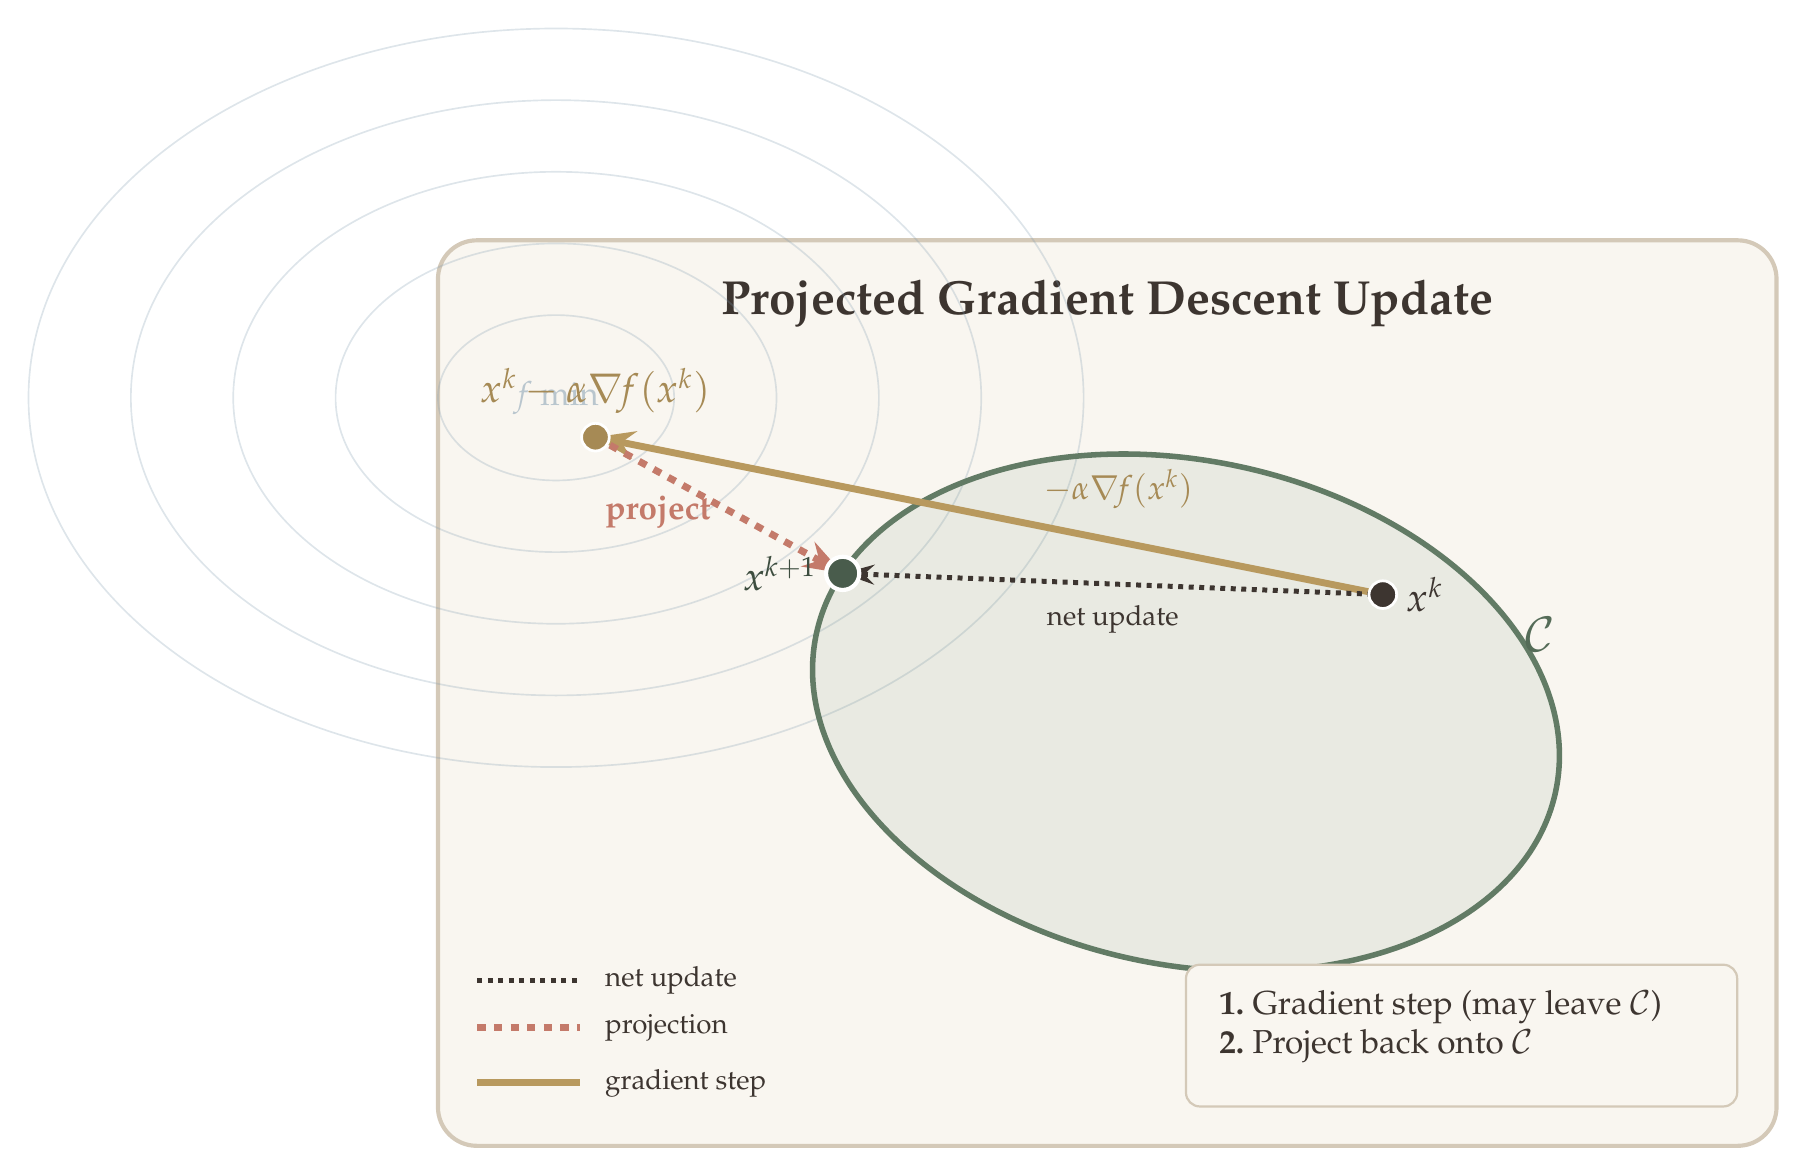
\begin{tikzpicture}[>={Stealth[length=4mm, width=3mm]}]

% Background
\fill[cream, rounded corners=14pt] (-3.5,-2.0) rectangle (13.5,9.5);
\draw[border, line width=1.5pt, rounded corners=14pt] (-3.5,-2.0) rectangle (13.5,9.5);

% Title
\node[text=dkbrown, font=\LARGE\bfseries] at (5.0,8.7)
  {Projected Gradient Descent Update};

% Contour lines of f (centered upper-left, outside C — the unconstrained min is there)
\foreach \r in {1.5, 2.8, 4.1, 5.4, 6.7} {
  \draw[stblue, line width=0.6pt, opacity=0.25]
    (-2.0,7.5) ellipse ({\r*1.0} and {\r*0.7});
}
\node[text=stblue, font=\large, opacity=0.5] at (-2.0,7.5) {$f$ min};

% Convex set C (large ellipse, tilted)
\begin{scope}[rotate around={-12:(6.0,3.5)}]
  \fill[sage, opacity=0.12] (6.0,3.5) ellipse (4.8cm and 3.2cm);
  \draw[sage!80!black, line width=2pt] (6.0,3.5) ellipse (4.8cm and 3.2cm);
\end{scope}

% Label C
\node[text=sage!70!black, font=\LARGE\bfseries] at (10.5,4.5) {$\mathcal{C}$};

% === Geometry: wide triangle so all three arrows are clearly separated ===
% x^k: inside C, right side
\coordinate (xk) at (8.5,5.0);
% Gradient step: goes upper-left toward unconstrained min, well outside C
\coordinate (gradstep) at (-1.5,7.0);
% x^{k+1}: EXACTLY on the ellipse boundary (parametric t=165 degrees)
\coordinate (xk1) at (1.64,5.27);

% --- Step 1: Gradient step arrow (solid gold) ---
\draw[rwgold, line width=2.5pt, -{Stealth[length=5mm, width=3.5mm]}]
  (xk) -- (gradstep);
\node[text=rwgold!90!black, font=\large\bfseries, above right=2pt]
  at ($(xk)!0.45!(gradstep)$) {$-\alpha\nabla\!f(x^k)$};

% --- Step 2: Projection arrow (dashed terracotta) ---
\draw[terracotta, line width=2.5pt, dashed, -{Stealth[length=5mm, width=3.5mm]}]
  (gradstep) -- (xk1);
\node[text=terracotta, font=\large\bfseries, left=4pt]
  at ($(gradstep)!0.55!(xk1)$) {project};

% --- Net update: dotted dark arrow from x^k to x^{k+1} ---
\draw[dkbrown, line width=1.8pt, dotted, -{Stealth[length=4mm, width=2.5mm]}]
  (xk) -- (xk1);
\node[text=dkbrown, font=\normalsize, below=4pt]
  at ($(xk)!0.5!(xk1)$) {net update};

% --- Points (large, high contrast) ---
\fill[dkbrown] (xk) circle (5pt);
\draw[white, line width=1pt] (xk) circle (5pt);
\node[text=dkbrown, font=\Large\bfseries, right=5pt] at (xk) {$x^k$};

\fill[rwgold!90!black] (gradstep) circle (5pt);
\draw[white, line width=1pt] (gradstep) circle (5pt);
\node[text=rwgold!90!black, font=\Large\bfseries, above=5pt] at (gradstep)
  {$x^k - \alpha\nabla\!f(x^k)$};

\fill[sage!60!black] (xk1) circle (6pt);
\draw[white, line width=1.5pt] (xk1) circle (6pt);
\node[text=sage!50!black, font=\Large\bfseries, left=6pt] at (xk1) {$x^{k+1}$};

% --- Annotation box ---
\fill[cream, rounded corners=5pt] (6.0,-1.5) rectangle (13.0,0.3);
\draw[border, line width=0.8pt, rounded corners=5pt] (6.0,-1.5) rectangle (13.0,0.3);
\node[text=dkbrown, font=\large, align=left, anchor=north west] at (6.3,0.1)
  {\textbf{1.}\ Gradient step (may leave $\mathcal{C}$)\\
   \textbf{2.}\ Project back onto $\mathcal{C}$};

% --- Legend: line styles ---
\draw[rwgold, line width=2.5pt] (-3.0,-1.2) -- (-1.7,-1.2);
\node[text=dkbrown, font=\normalsize, right] at (-1.5,-1.2) {gradient step};
\draw[terracotta, line width=2.5pt, dashed] (-3.0,-0.5) -- (-1.7,-0.5);
\node[text=dkbrown, font=\normalsize, right] at (-1.5,-0.5) {projection};
\draw[dkbrown, line width=1.8pt, dotted] (-3.0,0.1) -- (-1.7,0.1);
\node[text=dkbrown, font=\normalsize, right] at (-1.5,0.1) {net update};

\end{tikzpicture}
\end{document}
